\documentclass[12pt,a4paper]{article}

% =========================
% Packages
% =========================
\usepackage[utf8]{inputenc}
\usepackage[T1]{fontenc}
\usepackage[french]{babel}
\usepackage{amsmath, amssymb}
\usepackage{geometry}
\usepackage{fancyhdr}
\usepackage{lastpage}
\usepackage{xcolor}
\usepackage{listings}

\lstdefinestyle{matlabstyle}{
	language=Matlab,
	basicstyle=\ttfamily\small,
	keywordstyle=\color{blue},
	commentstyle=\color{green!50!black},
	stringstyle=\color{red!60!black},
	numbers=left,
	numberstyle=\tiny,
	stepnumber=1,
	numbersep=8pt,
	frame=single,
	breaklines=true,
	showstringspaces=false,
	tabsize=4
}
\usepackage{lmodern}
\usepackage{tikz}
\usepackage{float}
\usetikzlibrary{arrows.meta}
% =========================
% Mise en page
% =========================
\geometry{
	left=2.5cm,
	right=2.5cm,
	top=2.5cm,
	bottom=2.5cm
}

% =========================
% En-tête et pied de page
% =========================
\pagestyle{fancy}
\fancyhf{}

\fancyhead[L]{\textbf{TP -- Différences finies}}
\fancyhead[R]{\textbf{Problème de Poisson}}

\fancyfoot[L]{{\footnotesize Université de Yaoundé I / ENSPY-MMCS}}
\fancyfoot[C]{\thepage\ sur \pageref{LastPage}}
\fancyfoot[R]{{\footnotesize Méthodes numériques pour les EDP}}

\renewcommand{\headrulewidth}{0.4pt}
\renewcommand{\footrulewidth}{0.4pt}

\begin{document}
	
	\tableofcontents
	\newpage
	
	\section*{Introduction}
	\addcontentsline{toc}{section}{Introduction}
	
	Ce travail porte sur la résolution numérique d'un problème de Poisson posé sur
	le domaine carré $\Omega=]0,1[\times]0,1[$. L'objectif principal est d'utiliser
	la méthode des différences finies afin d'approcher la solution du problème à
	partir d'un maillage uniforme du domaine.
	
	Dans un premier temps, on établit le schéma aux différences finies associé au
	problème en déterminant le second membre, les conditions aux limites, la
	discrétisation du domaine ainsi que la forme matricielle du système linéaire.
	Ensuite, la solution numérique obtenue est comparée graphiquement à la solution
	analytique connue. Cette comparaison permet de vérifier visuellement la qualité
	de l'approximation.
	
	On étudie également l'erreur commise pour plusieurs valeurs du nombre de points
	intérieurs $N$, ainsi que le conditionnement de la matrice du système. Enfin,
	une analyse en échelle log-log permet d'estimer l'ordre de convergence de la
	méthode numérique.
	\newpage
	
	\section{Écriture du schéma aux différences finies}
	
	On considère le problème de Poisson suivant :
	\begin{equation*}
	\begin{cases}
	-\Delta u(x,y)=f(x,y), & (x,y)\in \Omega=]0,1[\times]0,1[,\\
	u(x,y)=g(x,y), & (x,y)\in \partial\Omega.
	\end{cases}
	\end{equation*}
	
	La solution exacte donnée est :
	\begin{equation*}
	u_{\mathrm{ex}}(x,y)
	=
	\cos\bigl(\pi(x+y)\bigr)\sin\bigl(\pi(x-y)\bigr).
	\end{equation*}
	
	\subsection{Détermination du second membre $f$}
	
	D'après l'identité trigonométrique suivante :
	\begin{equation*}
	\sin(b)\cos(a)
	=
	\frac{1}{2}\left[\sin(b+a)+\sin(b-a)\right].
	\end{equation*}
	
	Où :
	\begin{equation*}
	a=\pi(x+y),
	\qquad
	b=\pi(x-y).
	\end{equation*}
	
	On a :
	\begin{equation*}
	u_{\mathrm{ex}}(x,y)
	=
	\cos\bigl(\pi(x+y)\bigr)\sin\bigl(\pi(x-y)\bigr).
	\end{equation*}
	\begin{equation*}
	u_{\mathrm{ex}}(x,y)
	=
	\frac{1}{2}
	\left[
	\sin(2\pi x)
	-
	\sin(2\pi y)
	\right].
	\end{equation*}
	
	Calcul des dérivées secondes :
	\begin{equation*}
	\frac{\partial^2 u_{\mathrm{ex}}}{\partial x^2}
	=
	-2\pi^2 \sin(2\pi x),
	\end{equation*}
	
	et :
	\begin{equation*}
	\frac{\partial^2 u_{\mathrm{ex}}}{\partial y^2}
	=
	2\pi^2 \sin(2\pi y).
	\end{equation*}
	
	Donc :
	\begin{equation*}
	\Delta u_{\mathrm{ex}}
	=
	-2\pi^2 \sin(2\pi x)
	+
	2\pi^2 \sin(2\pi y).
	\end{equation*}
	
	Comme le problème vérifie :
	\begin{equation*}
	-\Delta u=f,
	\end{equation*}
	
	on obtient :
	\begin{equation*}
	\boxed{
		f(x,y)
		=
		2\pi^2\left[\sin(2\pi x)-\sin(2\pi y)\right].
	}
	\end{equation*}
	
	\subsection{Conditions aux limites}
	
	Les conditions aux limites sont obtenues à partir de la solution exacte :
	\begin{equation*}
	g(x,y)=u_{\mathrm{ex}}(x,y),
	\qquad (x,y)\in \partial\Omega.
	\end{equation*}
	
	Le domaine est le carré :
	\begin{equation*}
	\Omega=]0,1[\times]0,1[.
	\end{equation*}
	
	Il possède quatre bords.
	
	\subsubsection*{Bord gauche : \(x=0\)}
	
	Pour \(y\in[0,1]\), on a :
	\begin{equation*}
	u(0,y)
	=
	g(0,y)
	=
	\cos(\pi y)\sin(-\pi y).
	\end{equation*}
	
	Donc :
	\begin{equation*}
	\boxed{
		g(0,y)
		=
		-\cos(\pi y)\sin(\pi y).
	}
	\end{equation*}
	
	\subsubsection*{Bord droit : \(x=1\)}
	
	Pour \(y\in[0,1]\), on a :
	\begin{equation*}
	u(1,y)
	=
	g(1,y)
	=
	\cos\bigl(\pi(1+y)\bigr)
	\sin\bigl(\pi(1-y)\bigr).
	\end{equation*}
	
	Donc :
	\begin{equation*}
	\boxed{
		g(1,y)
		=
		\cos\bigl(\pi(1+y)\bigr)
		\sin\bigl(\pi(1-y)\bigr).
	}
	\end{equation*}
	
	\subsubsection*{Bord inférieur : \(y=0\)}
	
	Pour \(x\in[0,1]\), on a :
	\begin{equation*}
	u(x,0)
	=
	g(x,0)
	=
	\cos(\pi x)\sin(\pi x).
	\end{equation*}
	
	Donc :
	\begin{equation*}
	\boxed{
		g(x,0)
		=
		\cos(\pi x)\sin(\pi x).
	}
	\end{equation*}
	
	\subsubsection*{Bord supérieur : \(y=1\)}
	
	Pour \(x\in[0,1]\), on a :
	\begin{equation*}
	u(x,1)
	=
	g(x,1)
	=
	\cos\bigl(\pi(x+1)\bigr)
	\sin\bigl(\pi(x-1)\bigr).
	\end{equation*}
	
	Donc :
	\begin{equation*}
	\boxed{
		g(x,1)
		=
		\cos\bigl(\pi(x+1)\bigr)
		\sin\bigl(\pi(x-1)\bigr).
	}
	\end{equation*}
	
	Ainsi, les conditions aux limites sont :
	\begin{equation*}
	\boxed{
		\begin{cases}
		u(0,y)=g(0,y),\\
		u(1,y)=g(1,y),\\
		u(x,0)=g(x,0),\\
		u(x,1)=g(x,1).
		\end{cases}
	}
	\end{equation*}
	
	\subsection{Discrétisation du domaine}
	
	Soit un entier \(N\) représentant le nombre de points intérieurs dans chaque direction.
	
	On pose le pas du maillage $h$ comme suit :
	\begin{equation*}
	h=\frac{1}{N+1}.
	\end{equation*}
	
	Les points intérieurs sont :
	\begin{equation*}
	x_i=ih,
	\qquad
	y_j=jh,
	\end{equation*}
	
	avec :
	\begin{equation*}
	i,j=1,\dots,N.
	\end{equation*}
	
	On note :
	\begin{equation*}
	u_{i,j}\simeq u(x_i,y_j).
	\end{equation*}
	
	Les points du bord sont :
	\begin{equation*}
	x_0=0,
	\qquad
	x_{N+1}=1,
	\end{equation*}
	
	et :
	\begin{equation*}
	y_0=0,
	\qquad
	y_{N+1}=1.
	\end{equation*}
	
%	---------------------------------------------------------------------------
	\begin{figure}[H]
		\centering
		\begin{tikzpicture}[scale=1.1]
		
		% Taille du maillage : ici exemple avec N=4 points intérieurs
		\def\N{5} % nombre d'intervalles = N+1 si N=4 points intérieurs
		
		% Grille
		\draw[step=1cm, gray!50, thin] (0,0) grid (\N,\N);
		
		% Bord du domaine
		\draw[thick] (0,0) rectangle (\N,\N);
		
		% Points du bord en rouge
		\foreach \i in {0,...,\N} {
			\fill[red] (\i,0) circle (2.2pt);
			\fill[red] (\i,\N) circle (2.2pt);
			\fill[red] (0,\i) circle (2.2pt);
			\fill[red] (\N,\i) circle (2.2pt);
		}
		
		% Points intérieurs en bleu
		\foreach \i in {1,...,4} {
			\foreach \j in {1,...,4} {
				\fill[blue] (\i,\j) circle (2.2pt);
			}
		}
		
		% Quelques labels de points
		\node[below left] at (0,0) {$ (0,0)$};
		\node[below right] at (\N,0) {$ (1,0)$};
		\node[above left] at (0,\N) {$ (0,1)$};
		\node[above right] at (\N,\N) {$ (1,1)$};
		
		% Labels axes
		\draw[-Latex, thick] (-0.5,0) -- (\N+0.7,0) node[right] {$x$};
		\draw[-Latex, thick] (0,-0.5) -- (0,\N+0.7) node[above] {$y$};
		
		% Exemple de point intérieur
		\fill[blue] (2,3) circle (2.5pt);
		\node[right] at (2,3) {$u_{i,j}$};
		
		% Exemple de point de bord
		\fill[red] (0,3) circle (2.5pt);
		\node[left] at (0,3) {$g(0,y_j)$};
		
		% Légende manuelle
		\fill[blue] (6.8,4.5) circle (2.2pt);
		\node[right] at (7.0,4.5) {Point intérieur : inconnue $u_{i,j}$};
		
		\fill[red] (6.8,3.8) circle (2.2pt);
		\node[right] at (7.0,3.8) {Point du bord : valeur connue par $g$};
		
		\end{tikzpicture}
		\caption{Illustration du maillage uniforme du domaine $\Omega=[0,1]\times[0,1]$. Les points du bord, en rouge, correspondent aux valeurs connues imposées par les conditions aux limites, tandis que les points intérieurs, en bleu, représentent les inconnues du problème discret.}
		\label{fig:maillage_2D}
	\end{figure}


La figure \ref{fig:maillage_2D} représente le maillage uniforme utilisé pour discrétiser le domaine $\Omega=[0,1]\times[0,1]$. Les points situés sur le bord du domaine correspondent aux conditions aux limites de Dirichlet et leurs valeurs sont donc connues à partir de la fonction $g$. En revanche, les points intérieurs constituent les inconnues du problème discret. Le schéma aux différences finies est appliqué sur ces points intérieurs afin de construire le système linéaire $AU=b$.

\paragraph{NB:}Pour des raisons de lisibilité, la figure ci-dessus illustre le cas d’un maillage comportant un nombre réduit de points intérieurs. Le principe reste identique pour des valeurs plus grandes de $N$.
	
	
	
	
	
	\subsection{Approximation du Laplacien}
	
	Le Laplacien est défini par :
	\begin{equation*}
	\Delta u
	=
	\frac{\partial^2 u}{\partial x^2}
	+
	\frac{\partial^2 u}{\partial y^2}.
	\end{equation*}
	%-------------------------------------------------------------------------------
	
	L'approximation du Laplacien au point intérieur $(x_i,y_j)$ repose sur un stencil
	à cinq points. Ce stencil utilise la valeur de la fonction au point central
	$u_{i,j}$ ainsi que les valeurs aux quatre points voisins :
	$u_{i-1,j}$, $u_{i+1,j}$, $u_{i,j-1}$ et $u_{i,j+1}$.
	
	La figure \ref{fig:stencil_5_points} illustre localement les points utilisés
	dans le schéma aux différences finies.
%------------------------------------------------------------------------------	
	
	En utilisant un schéma centré d'ordre \(2\), on obtient:
	
	Dans la direction \(x\) :
	\begin{equation*}
	\frac{\partial^2 u}{\partial x^2}(x_i,y_j)
	\simeq
	\frac{u_{i+1,j}-2u_{i,j}+u_{i-1,j}}{h^2}.
	\end{equation*}
	
	Dans la direction \(y\) :
	\begin{equation*}
	\frac{\partial^2 u}{\partial y^2}(x_i,y_j)
	\simeq
	\frac{u_{i,j+1}-2u_{i,j}+u_{i,j-1}}{h^2}.
	\end{equation*}
	
	Donc :
	\begin{equation*}
	\Delta u(x_i,y_j)
	\simeq
	\frac{
		u_{i+1,j}
		+
		u_{i-1,j}
		+
		u_{i,j+1}
		+
		u_{i,j-1}
		-
		4u_{i,j}
	}{h^2}.
	\end{equation*}
	
	Comme :
	\begin{equation*}
	-\Delta u=f,
	\end{equation*}
	
	on obtient :
	\begin{equation*}
	\frac{
		4u_{i,j}
		-
		u_{i-1,j}
		-
		u_{i+1,j}
		-
		u_{i,j-1}
		-
		u_{i,j+1}
	}{h^2}
	=
	f(x_i,y_j).
	\end{equation*}
	
	En multipliant par \(h^2\), on obtient le schéma discret suivant:
	\begin{equation*}
	\boxed{
		4u_{i,j}
		-
		u_{i-1,j}
		-
		u_{i+1,j}
		-
		u_{i,j-1}
		-
		u_{i,j+1}
		=
		h^2 f(x_i,y_j).
	}
	\end{equation*}
	
	
	
		
	
	
	\begin{figure}[H]
		\centering
		\begin{tikzpicture}[scale=1.25]
		
		% Grille locale
		\draw[step=1cm, gray!40, thin] (-1.5,-1.5) grid (1.5,1.5);
		
		% Axes locaux
		\draw[-Latex, thick] (-1.8,0) -- (1.9,0) node[right] {$x$};
		\draw[-Latex, thick] (0,-1.8) -- (0,1.9) node[above] {$y$};
		
		% Points voisins
		\fill[blue] (0,0) circle (3pt);
		\fill[orange] (-1,0) circle (3pt);
		\fill[orange] (1,0) circle (3pt);
		\fill[orange] (0,-1) circle (3pt);
		\fill[orange] (0,1) circle (3pt);
		
		% Labels des points
		\node[below right] at (0,0) {$u_{i,j}$};
		
		\node[below] at (-1,0) {$u_{i-1,j}$};
		\node[below] at (1,0) {$u_{i+1,j}$};
		\node[right] at (0,1) {$u_{i,j+1}$};
		\node[right] at (0,-1) {$u_{i,j-1}$};
		
		% Lignes du stencil
		\draw[thick, dashed] (-1,0) -- (1,0);
		\draw[thick, dashed] (0,-1) -- (0,1);
		
		% Espacement h
		\draw[<->] (-1,-1.35) -- (0,-1.35);
		\node[below] at (-0.5,-1.35) {$h$};
		
		\draw[<->] (0,-1.35) -- (1,-1.35);
		\node[below] at (0.5,-1.35) {$h$};
		
		\draw[<->] (1.35,0) -- (1.35,1);
		\node[right] at (1.35,0.5) {$h$};
		
		\draw[<->] (1.35,-1) -- (1.35,0);
		\node[right] at (1.35,-0.5) {$h$};
		
		% Légende
		\fill[blue] (2.4,1.1) circle (3pt);
		\node[right] at (2.6,1.1) {Point central};
		
		\fill[orange] (2.4,0.55) circle (3pt);
		\node[right] at (2.6,0.55) {Voisins utilisés};
		
		\end{tikzpicture}
		\caption{Stencil à cinq points utilisé pour approximer le Laplacien au point intérieur $(x_i,y_j)$.}
		\label{fig:stencil_5_points}
	\end{figure}
	
	
	
	Le point $u_{i,j}$ représente l'inconnue principale sur laquelle le schéma est
	appliqué. Les quatre points voisins interviennent dans l'approximation des
	dérivées secondes selon les directions $x$ et $y$. Comme le pas du maillage est
	identique dans les deux directions, la contribution de chaque voisin apparaît
	avec le même coefficient dans le schéma discret.
	
	Cette représentation permet de comprendre l'origine du schéma :
	\[
	4u_{i,j}
	-
	u_{i-1,j}
	-
	u_{i+1,j}
	-
	u_{i,j-1}
	-
	u_{i,j+1}
	=
	h^2 f(x_i,y_j).
	\]
	Le coefficient $4$ devant $u_{i,j}$ provient de la somme des deux dérivées
	secondes discrétisées, tandis que les coefficients $-1$ correspondent aux quatre
	voisins directs.
	
	
	\subsection{Gestion des conditions aux limites dans le schéma}
	
	Le schéma précédent contient les voisins :
	\begin{equation*}
	u_{i-1,j},
	\qquad
	u_{i+1,j},
	\qquad
	u_{i,j-1},
	\qquad
	u_{i,j+1}.
	\end{equation*}
	
	Si ces voisins sont dans le domaine intérieur, ils restent des inconnues du système.
	
	Mais si un voisin tombe sur le bord, sa valeur est connue grâce aux conditions aux limites. Cette valeur est alors déplacée dans le second membre.
	
	\subsubsection*{Contribution du bord gauche}
	
	Si \(i=1\), alors :
	\begin{equation*}
	u_{i-1,j}=u_{0,j}=g(0,y_j).
	\end{equation*}
	
	Le schéma devient :
	\begin{equation*}
	4u_{1,j}
	-
	u_{2,j}
	-
	u_{1,j-1}
	-
	u_{1,j+1}
	=
	h^2 f(x_1,y_j)
	+
	g(0,y_j).
	\end{equation*}
	
	\subsubsection*{Contribution du bord droit}
	
	Si \(i=N\), alors :
	\begin{equation*}
	u_{i+1,j}=u_{N+1,j}=g(1,y_j).
	\end{equation*}
	
	Le schéma devient :
	\begin{equation*}
	4u_{N,j}
	-
	u_{N-1,j}
	-
	u_{N,j-1}
	-
	u_{N,j+1}
	=
	h^2 f(x_N,y_j)
	+
	g(1,y_j).
	\end{equation*}
	
	\subsubsection*{Contribution du bord inférieur}
	
	Si \(j=1\), alors :
	\begin{equation*}
	u_{i,j-1}=u_{i,0}=g(x_i,0).
	\end{equation*}
	
	Le schéma devient :
	\begin{equation*}
	4u_{i,1}
	-
	u_{i-1,1}
	-
	u_{i+1,1}
	-
	u_{i,2}
	=
	h^2 f(x_i,y_1)
	+
	g(x_i,0).
	\end{equation*}
	
	\subsubsection*{Contribution du bord supérieur}
	
	Si \(j=N\), alors :
	\begin{equation*}
	u_{i,j+1}=u_{i,N+1}=g(x_i,1).
	\end{equation*}
	
	Le schéma devient :
	\begin{equation*}
	4u_{i,N}
	-
	u_{i-1,N}
	-
	u_{i+1,N}
	-
	u_{i,N-1}
	=
	h^2 f(x_i,y_N)
	+
	g(x_i,1).
	\end{equation*}
	

	\subsection{Mise sous forme matricielle}
	
	On regroupe les inconnues \(u_{i,j}\) dans un vecteur colonne \(U\) de taille \(N^2\).
	
	On peut choisir l'ordre suivant :
	\begin{equation*}
	U=
	\begin{pmatrix}
	u_{1,1}\\
	u_{2,1}\\
	\vdots\\
	u_{N,1}\\
	u_{1,2}\\
	u_{2,2}\\
	\vdots\\
	u_{N,N}
	\end{pmatrix}.
	\end{equation*}
	
	Le problème discret s'écrit alors :
	\begin{equation*}
	\boxed{
		AU=b.
	}
	\end{equation*}
	
	La matrice \(A\) est une matrice de taille \(N^2\times N^2\).
	
	Elle est donnée par blocs :
	\begin{equation*}
	A=
	\begin{pmatrix}
	T & -I & 0 & \cdots & 0\\
	-I & T & -I & \ddots & \vdots\\
	0 & -I & T & \ddots & 0\\
	\vdots & \ddots & \ddots & \ddots & -I\\
	0 & \cdots & 0 & -I & T
	\end{pmatrix},
	\end{equation*}
	
	où \(I\) est la matrice identité de taille \(N\times N\), et :
	\begin{equation*}
	T=
	\begin{pmatrix}
	4 & -1 & 0 & \cdots & 0\\
	-1 & 4 & -1 & \ddots & \vdots\\
	0 & -1 & 4 & \ddots & 0\\
	\vdots & \ddots & \ddots & \ddots & -1\\
	0 & \cdots & 0 & -1 & 4
	\end{pmatrix}.
	\end{equation*}
	
	
La résolution numérique revient donc à résoudre :
\begin{equation*}
\boxed{
	AU=b.
}
\end{equation*}




% Question 2


\section{Visualisation graphique de la solution analytique et numérique}

Dans cette partie, on compare graphiquement la solution analytique $u_{\mathrm{ex}}$
et la solution numérique $u_h$ obtenue par la méthode des différences finies.
L'objectif est de vérifier visuellement si le schéma numérique reproduit
correctement la forme générale de la solution exacte.

La comparaison est effectuée pour plusieurs valeurs du nombre de points
intérieurs du maillage :
\[
N = 4,\; 8,\; 32,\; 64.
\]

Lorsque $N$ augmente, le pas du maillage
\[
h = \frac{1}{N+1}
\]
diminue. Le maillage devient donc plus fin, ce qui doit normalement améliorer
la précision de la solution numérique.

\subsection{Visualisation pour $N=4$}

\begin{figure}[!htbp]
	\centering
	
	\begin{minipage}[c]{0.32\textwidth}
		\centering
		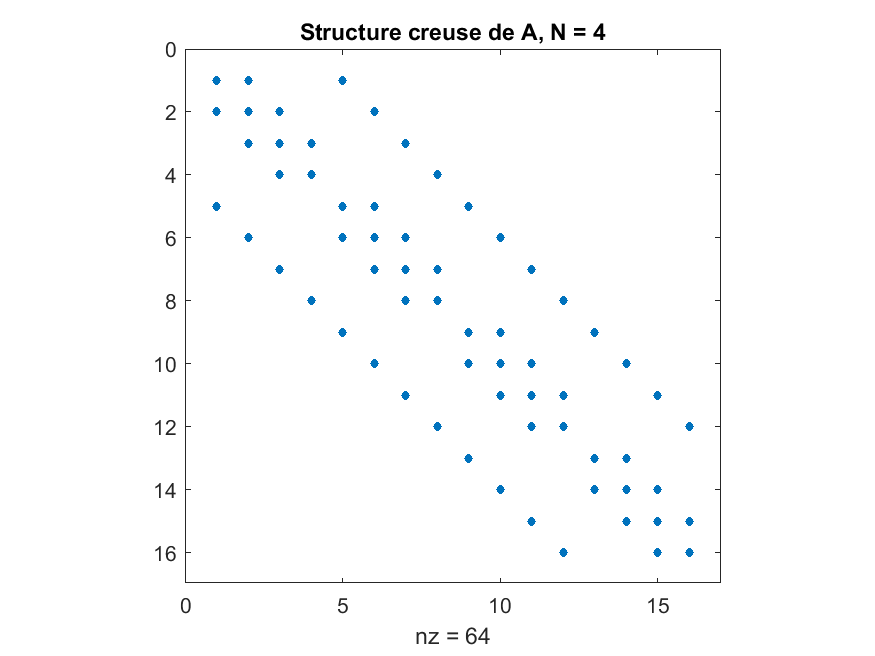
\includegraphics[width=\textwidth]{structure_matrice_A_N4.png}
		
		\vspace{0.2cm}
		{\small (a) Structure creuse de $A$.}
	\end{minipage}
	\hfill
	\begin{minipage}[c]{0.62\textwidth}
		\centering
		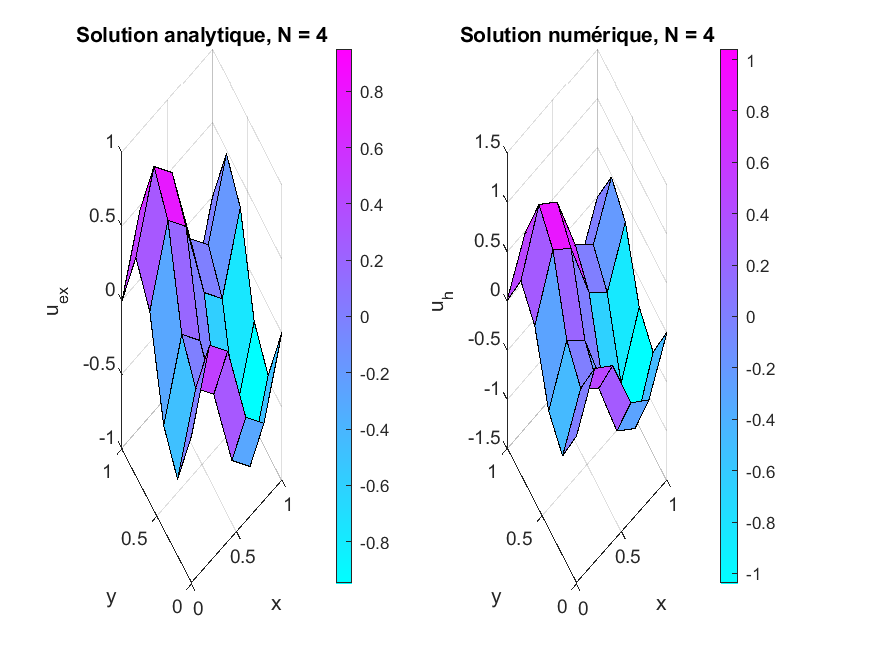
\includegraphics[width=\textwidth]{comparaison_solutions_N4.png}
		
		\vspace{0.2cm}
		{\small (b) Comparaison entre $u_{\mathrm{ex}}$ et $u_h$.}
	\end{minipage}
	
	\caption{Structure de la matrice $A$ et comparaison entre la solution analytique et la solution numérique pour $N=4$.}
	\label{fig:structure_solution_N4}
\end{figure}

Pour $N=4$, le maillage est très grossier. La solution numérique est calculée
sur un faible nombre de points intérieurs, ce qui limite sa capacité à
représenter correctement les variations de la solution analytique. La forme
générale de la solution est déjà visible, mais l'approximation reste peu
précise.

\subsection{Visualisation pour $N=8$}

\begin{figure}[!htbp]
	\centering
	
	\begin{minipage}[c]{0.32\textwidth}
		\centering
		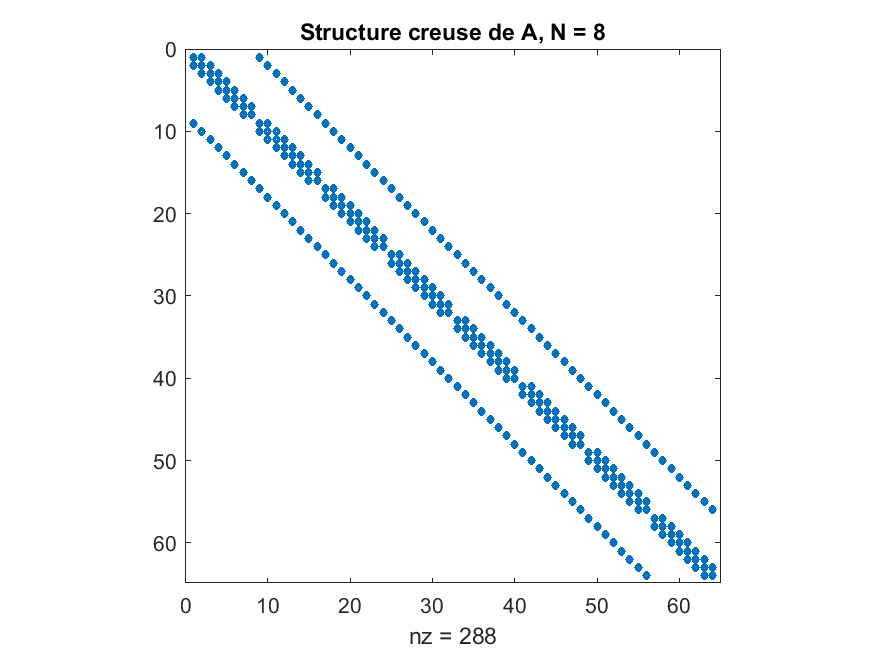
\includegraphics[width=\textwidth]{structure_matrice_A_N8.png}
		
		\vspace{0.2cm}
		{\small (a) Structure creuse de $A$.}
	\end{minipage}
	\hfill
	\begin{minipage}[c]{0.62\textwidth}
		\centering
		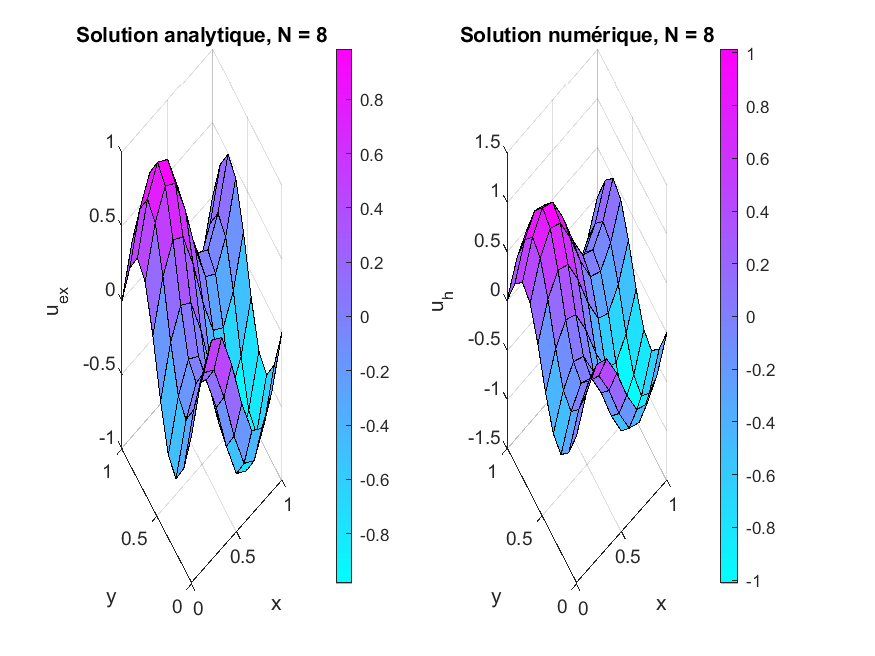
\includegraphics[width=\textwidth]{comparaison_solutions_N8.png}
		
		\vspace{0.2cm}
		{\small (b) Comparaison entre $u_{\mathrm{ex}}$ et $u_h$.}
	\end{minipage}
	
	\caption{Structure de la matrice $A$ et comparaison entre la solution analytique et la solution numérique pour $N=8$.}
	\label{fig:structure_solution_N8}
\end{figure}
Pour $N=8$, le maillage devient plus fin. La solution numérique commence à mieux
suivre la solution analytique. Les variations de la surface sont mieux
représentées que dans le cas $N=4$, même si des écarts restent encore visibles.

\subsection{Visualisation pour $N=32$}
\begin{figure}[!htbp]
	\centering
	
	\begin{minipage}[c]{0.32\textwidth}
		\centering
		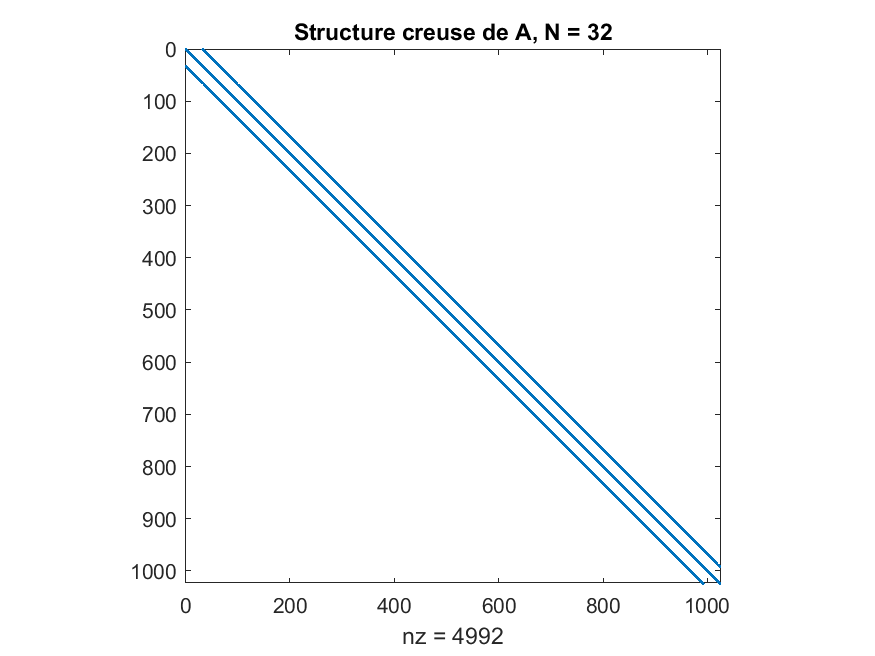
\includegraphics[width=\textwidth]{structure_matrice_A_N32.png}
		
		\vspace{0.2cm}
		{\small (a) Structure creuse de $A$.}
	\end{minipage}
	\hfill
	\begin{minipage}[c]{0.62\textwidth}
		\centering
		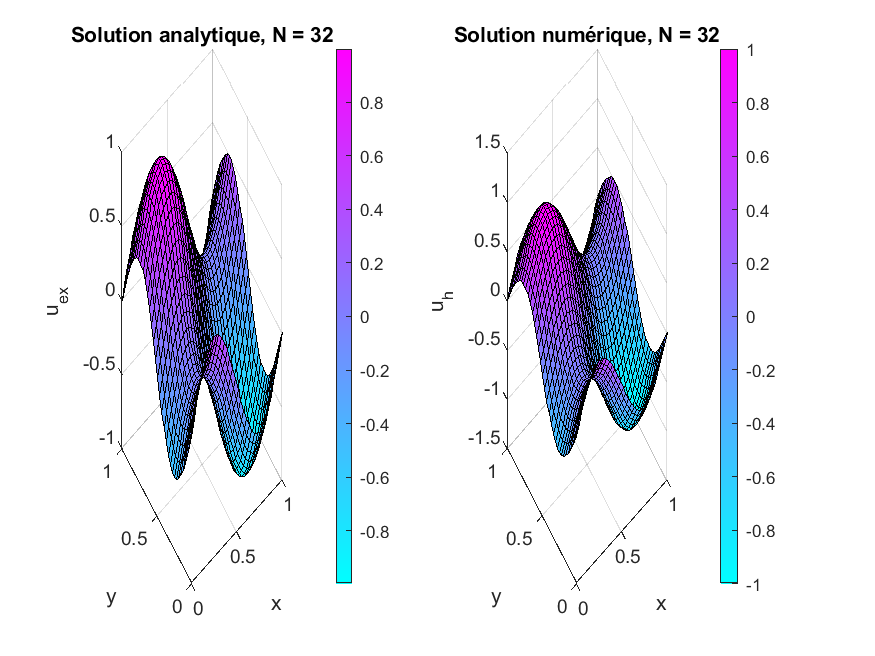
\includegraphics[width=\textwidth]{comparaison_solutions_N32.png}
		
		\vspace{0.2cm}
		{\small (b) Comparaison entre $u_{\mathrm{ex}}$ et $u_h$.}
	\end{minipage}
	
	\caption{Structure de la matrice $A$ et comparaison entre la solution analytique et la solution numérique pour $N=32$.}
	\label{fig:structure_solution_N32}
\end{figure}

Pour $N=32$, la solution numérique devient nettement plus proche de la solution
analytique. Les formes des deux surfaces sont presque identiques. Cela montre
que le schéma aux différences finies capture correctement le comportement de la
solution lorsque le maillage est suffisamment raffiné.

\subsection{Visualisation pour $N=64$}
\begin{figure}[!htbp]
	\centering
	
	\begin{minipage}[c]{0.32\textwidth}
		\centering
		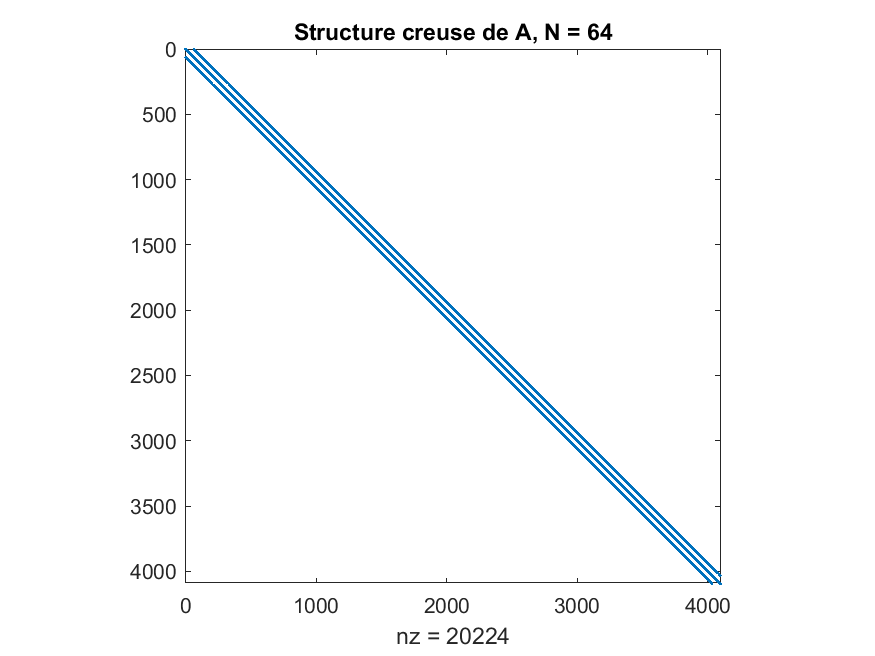
\includegraphics[width=\textwidth]{structure_matrice_A_N64.png}
		
		\vspace{0.2cm}
		{\small (a) Structure creuse de $A$.}
	\end{minipage}
	\hfill
	\begin{minipage}[c]{0.62\textwidth}
		\centering
		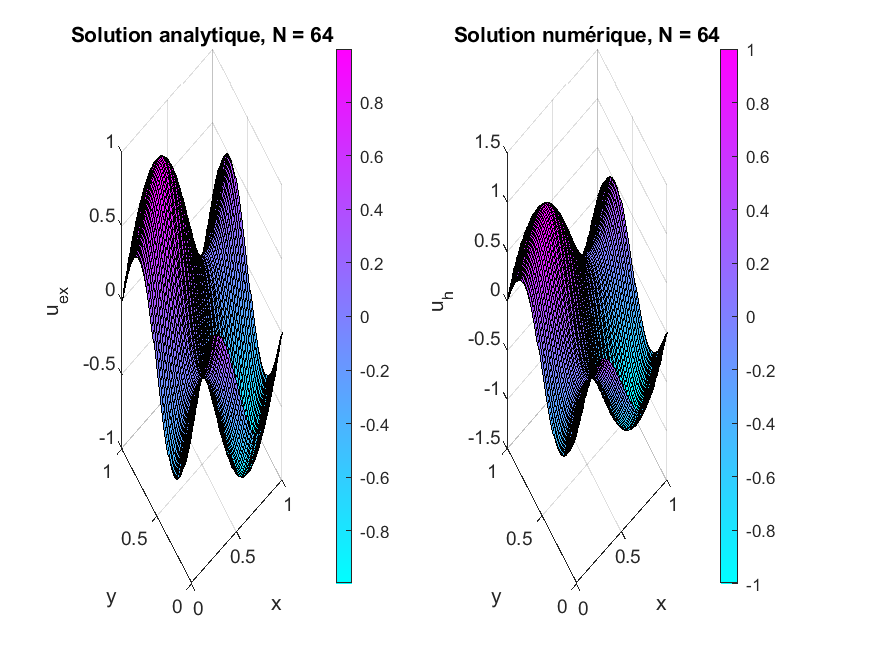
\includegraphics[width=\textwidth]{comparaison_solutions_N64.png}
		
		\vspace{0.2cm}
		{\small (b) Comparaison entre $u_{\mathrm{ex}}$ et $u_h$.}
	\end{minipage}
	
	\caption{Structure de la matrice $A$ et comparaison entre la solution analytique et la solution numérique pour $N=64$.}
	\label{fig:structure_solution_N64}
\end{figure}

Pour $N=64$, le maillage est très fin. La solution numérique est presque
confondue avec la solution analytique à l'échelle graphique. Les différences
restantes deviennent difficiles à observer directement sur les surfaces, ce qui
confirme l'amélioration de la précision lorsque le pas $h$ diminue.

\subsection{Interprétation générale}

Les différentes visualisations montrent que la solution numérique se rapproche
progressivement de la solution analytique lorsque $N$ augmente. Pour les petits
maillages, notamment $N=4$, l'approximation est encore grossière, car le nombre
de points de calcul est insuffisant. En revanche, pour $N=32$ et $N=64$, la
solution numérique reproduit très fidèlement la forme de la solution exacte.

Cette évolution est cohérente avec le comportement attendu du schéma aux
différences finies centré d'ordre $2$ utilisé pour approximer le Laplacien. En
raffinant le maillage, c'est-à-dire en diminuant le pas $h$, l'erreur de
discrétisation diminue et la solution numérique devient plus précise.

Il faut cependant noter que la superposition graphique ne signifie pas que
l'erreur est nulle. Même lorsque les deux surfaces semblent confondues, il
subsiste une erreur numérique. Celle-ci sera étudiée plus précisément dans la
partie suivante à travers la représentation graphique de l'erreur.




% Question 3: representation gra[hique de l'erreur



\section{Représentation graphique de l'erreur}

Dans cette partie, on représente graphiquement l'erreur absolue entre la solution
analytique $u_{\mathrm{ex}}$ et la solution numérique $u_h$. Cette erreur est
définie par :
\[
E_h(x_i,y_j)=\left|u_{\mathrm{ex}}(x_i,y_j)-u_h(x_i,y_j)\right|.
\]

L'objectif est d'observer la répartition spatiale de l'erreur sur le domaine
$\Omega=[0,1]\times[0,1]$ pour différentes valeurs de $N$. Lorsque le maillage
est raffiné, c'est-à-dire lorsque $N$ augmente et que le pas $h$ diminue, on
s'attend à ce que l'erreur numérique diminue.

\subsection{Erreur pour $N=4$}

\begin{figure}[!htbp]
	\centering
	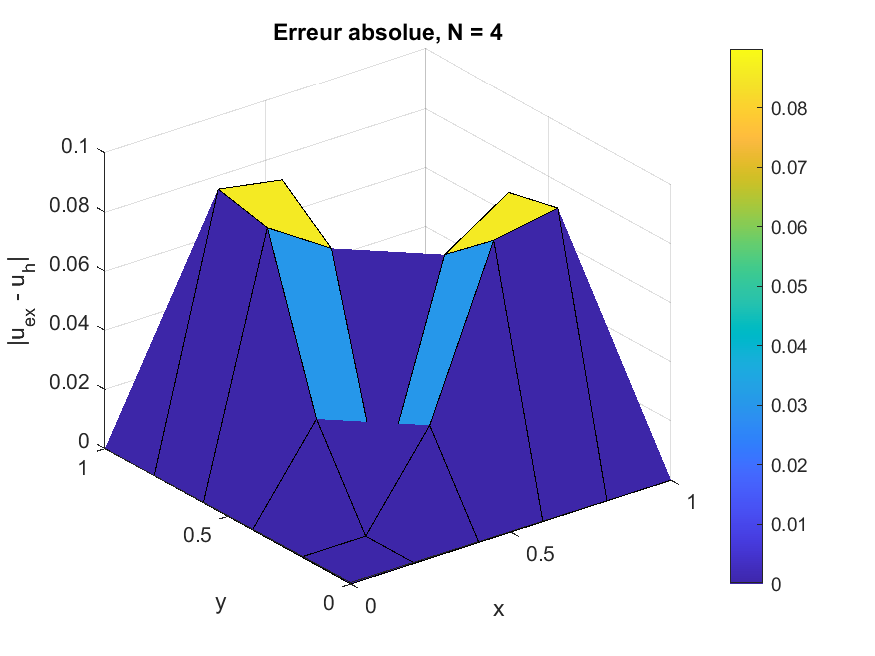
\includegraphics[width=0.75\textwidth]{erreur_absolue_N4.png}
	\caption{Erreur absolue entre la solution analytique et la solution numérique pour $N=4$.}
	\label{fig:erreur_N4}
\end{figure}

Pour $N=4$, le maillage est très grossier. L'erreur est donc relativement
importante, car la solution numérique est calculée avec peu de points
intérieurs. Les variations de la solution exacte sont encore mal capturées par
le schéma discret.

\subsection{Erreur pour $N=8$}

\begin{figure}[!htbp]
	\centering
	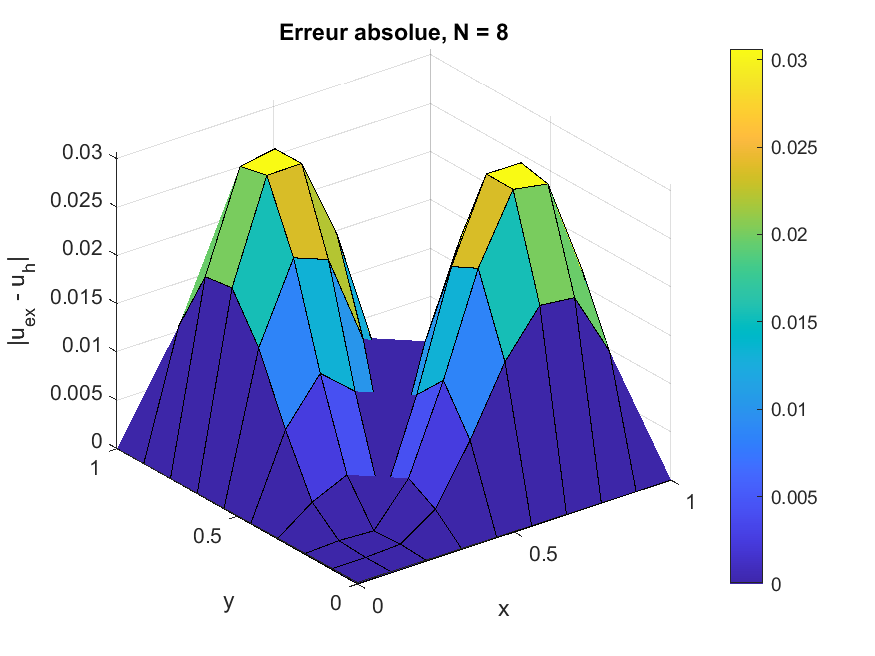
\includegraphics[width=0.75\textwidth]{erreur_absolue_N8.png}
	\caption{Erreur absolue entre la solution analytique et la solution numérique pour $N=8$.}
	\label{fig:erreur_N8}
\end{figure}

Pour $N=8$, le maillage est plus fin que dans le cas précédent. L'erreur diminue
globalement, car l'approximation numérique représente mieux les variations de la
solution analytique. On observe cependant que certaines zones du domaine restent
plus sensibles à l'erreur de discrétisation.

\subsection{Erreur pour $N=32$}

\begin{figure}[!htbp]
	\centering
	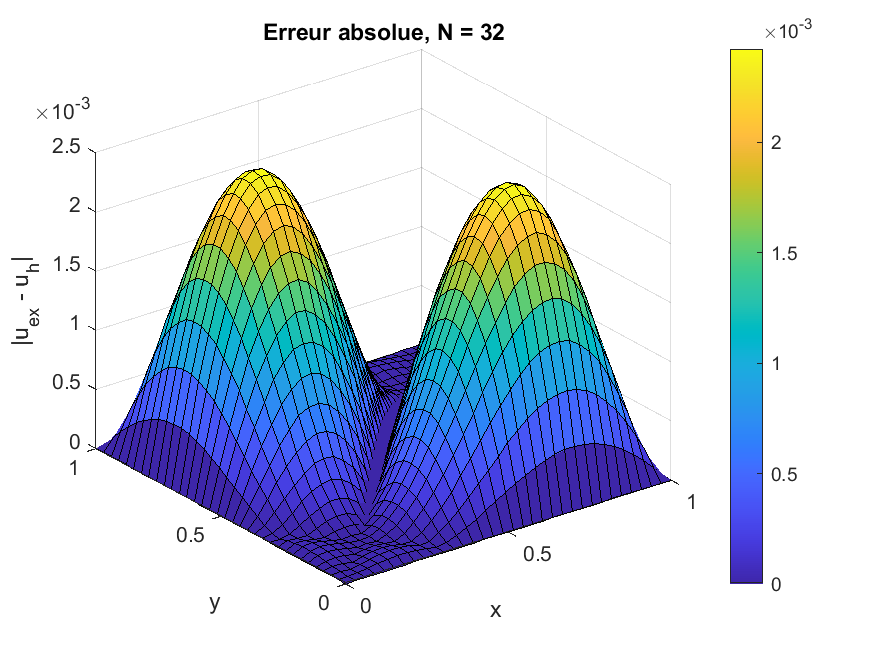
\includegraphics[width=0.75\textwidth]{erreur_absolue_N32.png}
	\caption{Erreur absolue entre la solution analytique et la solution numérique pour $N=32$.}
	\label{fig:erreur_N32}
\end{figure}

Pour $N=32$, l'erreur devient nettement plus faible. Le raffinement du maillage
permet au schéma aux différences finies de mieux approximer le Laplacien. La
solution numérique est alors beaucoup plus proche de la solution analytique sur
l'ensemble du domaine.

\subsection{Erreur pour $N=64$}

\begin{figure}[!htbp]
	\centering
	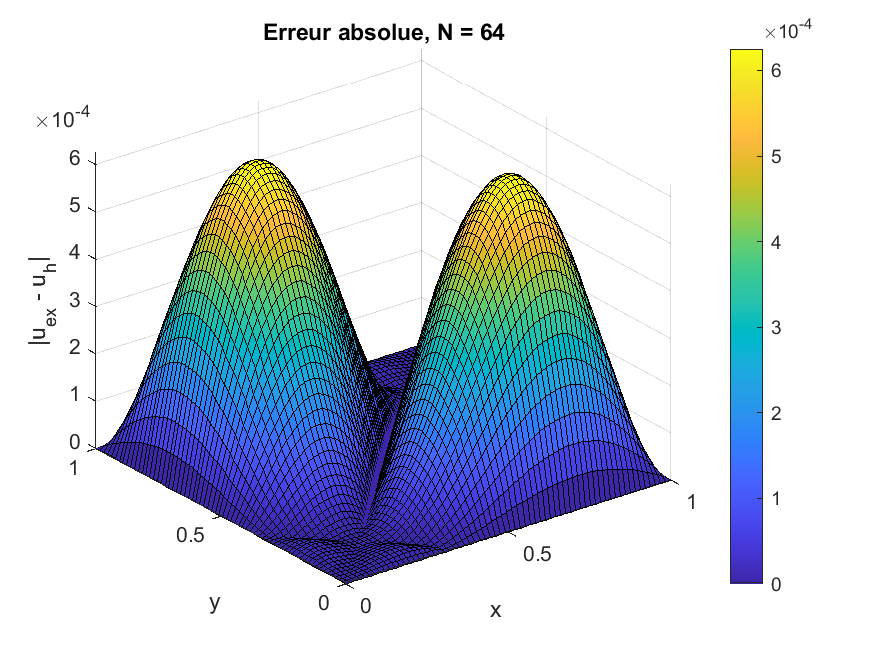
\includegraphics[width=0.75\textwidth]{erreur_absolue_N64.png}
	\caption{Erreur absolue entre la solution analytique et la solution numérique pour $N=64$.}
	\label{fig:erreur_N64}
\end{figure}

Pour $N=64$, l'erreur est encore plus faible. À cette échelle de maillage, la
solution numérique est très proche de la solution analytique. 

\subsection{Interprétation générale}

Les représentations graphiques de l'erreur montrent que l'erreur absolue diminue
lorsque le nombre de points intérieurs $N$ augmente. Cela confirme que le
raffinement du maillage améliore la précision de la solution numérique.

Ce comportement est cohérent avec le schéma centré d'ordre $2$ utilisé pour
approximer le Laplacien. En effet, lorsque le pas $h$ diminue, l'erreur de
discrétisation devient plus faible. La représentation graphique de l'erreur
permet donc de visualiser concrètement la convergence de la solution numérique
vers la solution analytique.

Il faut toutefois faire attention à l'échelle des couleurs utilisée dans les
figures. Deux surfaces d'erreur peuvent sembler visuellement proches alors que
leurs amplitudes maximales sont différentes. Pour comparer rigoureusement les
erreurs entre plusieurs valeurs de $N$, il est nécessaire de compléter cette
analyse graphique par le calcul de normes d'erreur, par exemple les normes
$L^\infty$ et $L^2$.



% Question 4

\section{Calcul du nombre de conditionnement de la matrice}

Dans cette partie, on étudie le nombre de conditionnement de la matrice $A$
obtenue après discrétisation du problème de Poisson. Le système linéaire à
résoudre est de la forme :
\[
AU=b.
\]

Le nombre de conditionnement d'une matrice mesure la sensibilité de la solution
du système linéaire aux petites perturbations du second membre ou aux erreurs
d'arrondi. Il est défini par :
\[
\operatorname{cond}(A)=\|A\|\,\|A^{-1}\|.
\]

Plus ce nombre est grand, plus le système est sensible numériquement. Dans ce
travail, le conditionnement est calculé pour plusieurs valeurs de $N$, avec :
\[
h=\frac{1}{N+1}.
\]

\subsection{Tableau récapitulatif des résultats}

Les résultats numériques obtenus sous MATLAB sont regroupés dans le tableau
suivant.

\begin{table}[!htbp]
	\centering
	\renewcommand{\arraystretch}{1.3}
	\begin{tabular}{c c c c c}
		\hline
		$N$ & $h$ & Conditionnement & Erreur\_$L^\infty$ & Erreur\_$L^2$ \\
		\hline
		$4$  & $0.2$       & $13.333$  & $0.089883$   & $0.048915$  \\
		$8$  & $0.11111$   & $46.295$  & $0.030609$   & $0.014864$  \\
			$16$ & $0.058824$  & $168.87$  & $0.0091176$  & $0.0041445$ \\
		$32$ & $0.030303$  & $640.36$  & $0.0024226$  & $0.0010982$ \\
		$64$ & $0.015385$  & $2488.6$  & $0.00062501$ & $0.00028295$ \\
		\hline
	\end{tabular}
	\caption{Tableau récapitulatif du conditionnement de la matrice $A$ et des erreurs numériques pour différentes valeurs de $N$.}
	\label{tab:resultats_conditionnement_erreurs}
\end{table}


\subsection{Interprétation des résultats}

D'après le tableau \ref{tab:resultats_conditionnement_erreurs}, on observe que
le nombre de conditionnement de la matrice $A$ augmente lorsque $N$ augmente.
Par exemple, il passe de $13.333$ pour $N=4$ à $2488.6$ pour $N=64$.

Cette évolution signifie que plus le maillage est raffiné, plus la matrice du
système devient mal conditionnée. Cela est attendu pour la discrétisation du
problème de Poisson par différences finies : lorsque le pas $h$ diminue, la
taille de la matrice augmente et le système linéaire devient plus sensible aux
erreurs numériques.

En parallèle, les erreurs $L^\infty$ et $L^2$ diminuent lorsque $N$ augmente.
L'erreur $L^\infty$ passe de $0.089883$ pour $N=4$ à $0.00062501$ pour $N=64$.
De même, l'erreur $L^2$ passe de $0.048915$ à $0.00028295$.

Ces résultats montrent donc deux phénomènes opposés. D'un côté, le raffinement
du maillage améliore la précision de la solution numérique. De l'autre côté, il
augmente le conditionnement de la matrice, ce qui rend la résolution du système
linéaire plus délicate numériquement.

Ainsi, l'augmentation de $N$ permet d'obtenir une solution plus précise, mais au
prix d'un système linéaire plus grand et plus sensible aux erreurs d'arrondi.

Afin de quantifier plus précisément la diminution des erreurs
lorsque le pas $h$ diminue, on étudie dans la partie suivante l'évolution des
erreurs $L^\infty$ et $L^2$ à l'aide d'une représentation en échelle logarithmique.



% question 5

\section{Courbes log-log des erreurs et estimation de l'ordre de convergence}

Dans cette partie, on étudie l'évolution des erreurs numériques en fonction du
pas du maillage $h$. Les erreurs considérées sont l'erreur en norme $L^\infty$
et l'erreur en norme $L^2$.

Les calculs sont effectués pour plusieurs valeurs de $N$ :
\[
N=4,\;8,\;16,\;32,\;64.
\]

Pour chaque valeur de $N$, le pas du maillage est donné par :
\[
h=\frac{1}{N+1}.
\]

L'objectif est de vérifier le comportement de convergence de la méthode des
différences finies lorsque le maillage est raffiné. Pour cela, on représente les
erreurs en fonction du pas $h$ dans une échelle logarithmique.

\subsection{Définition des erreurs}

L'erreur en norme $L^\infty$ est définie par :
\[
\|u_{\mathrm{ex}}-u_h\|_{L^\infty}
=
\max_{i,j}
\left|u_{\mathrm{ex}}(x_i,y_j)-u_h(x_i,y_j)\right|.
\]

Cette norme mesure l'erreur maximale obtenue sur l'ensemble du maillage.

L'erreur en norme $L^2$ est approximée par :
\[
\|u_{\mathrm{ex}}-u_h\|_{L^2}
\simeq
\left(
h^2
\sum_{i,j}
\left|u_{\mathrm{ex}}(x_i,y_j)-u_h(x_i,y_j)\right|^2
\right)^{1/2}.
\]

Cette norme donne une mesure globale de l'erreur sur le domaine.

\subsection{Représentation log-log des erreurs}

\begin{figure}[!htbp]
	\centering
	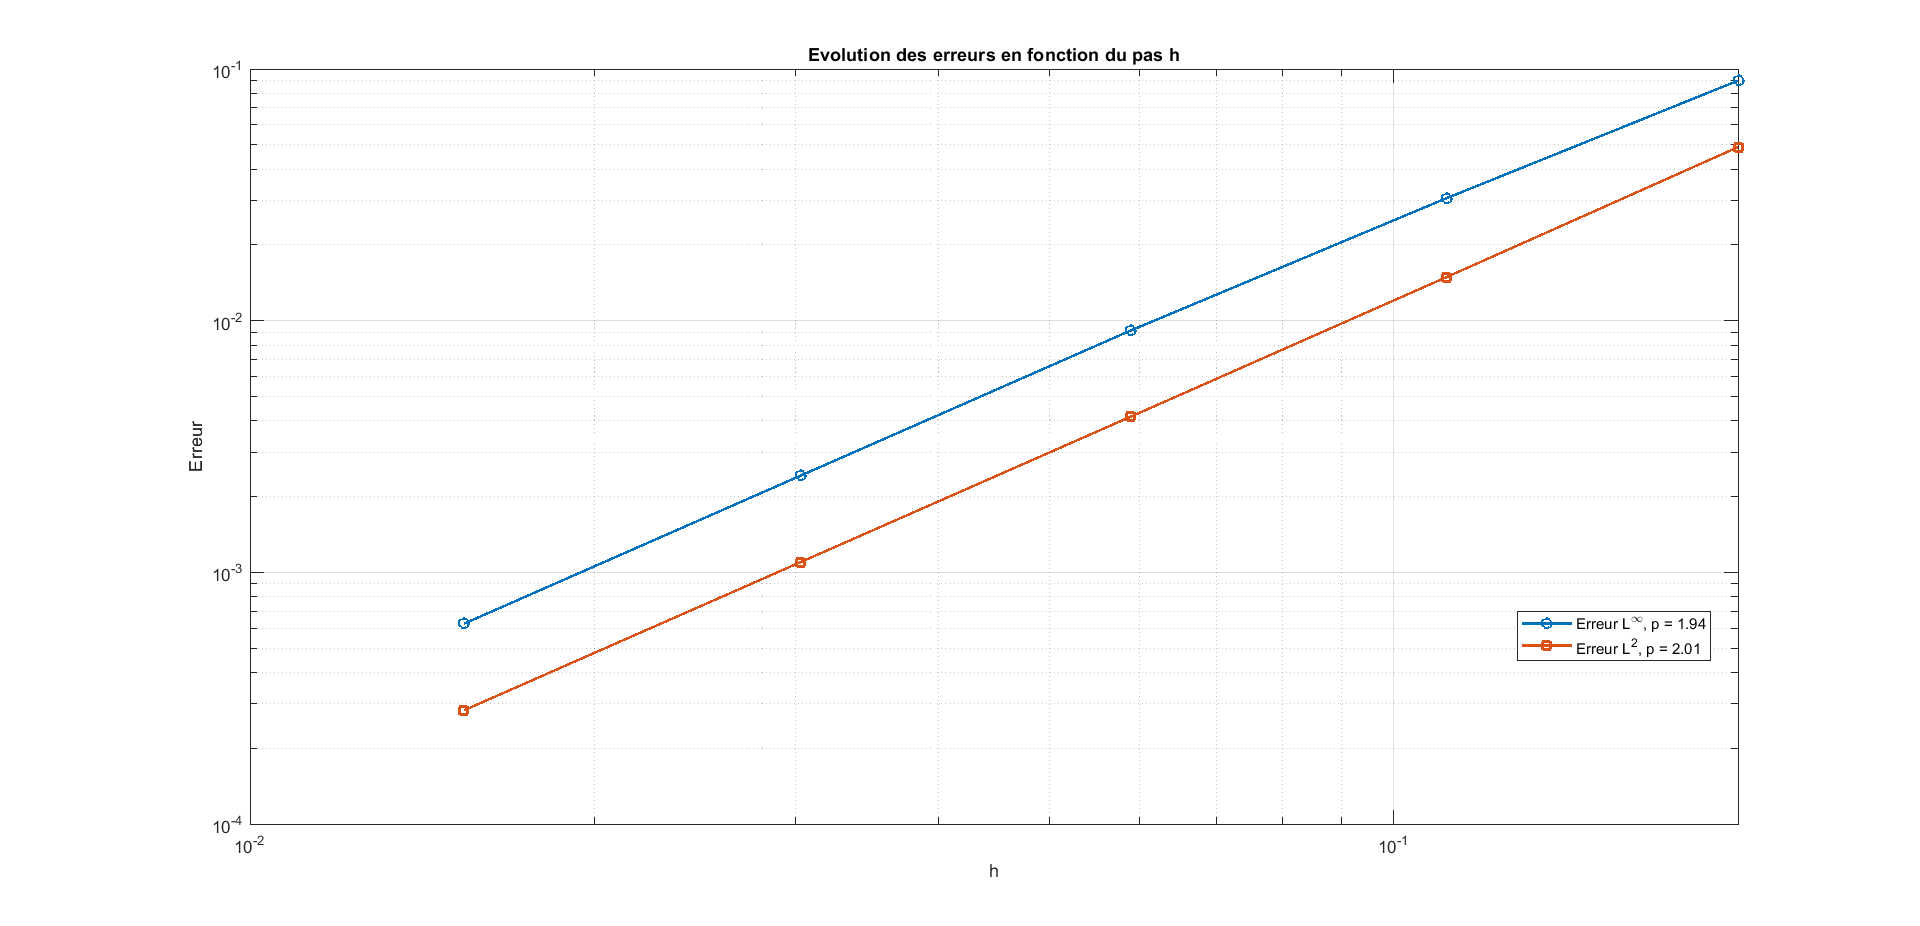
\includegraphics[width=0.75\textwidth]{courbes_loglog_erreurs.png}
	\caption{Courbes log-log des erreurs $L^\infty$ et $L^2$ en fonction du pas $h$.}
	\label{fig:courbes_loglog_erreurs}
\end{figure}

La figure \ref{fig:courbes_loglog_erreurs} représente les erreurs $L^\infty$ et
$L^2$ en fonction du pas $h$ en échelle log-log. Cette représentation permet
d'observer plus clairement la vitesse de décroissance des erreurs lorsque le
maillage est raffiné.

On observe que les deux erreurs diminuent lorsque $h$ diminue, c'est-à-dire
lorsque $N$ augmente. Cela confirme que la solution numérique converge vers la
solution analytique lorsque le maillage devient plus fin.

\subsection{Estimation de l'ordre de convergence}

Pour estimer l'ordre de convergence, on suppose que l'erreur suit une loi de la
forme :
\[
E(h) \simeq C h^p,
\]
où $C$ est une constante et $p$ représente l'ordre de convergence numérique.

En prenant le logarithme, on obtient :
\[
\log(E(h))
\simeq
\log(C)+p\log(h).
\]

Ainsi, dans une représentation log-log, l'ordre $p$ correspond à la pente de la
droite ajustée aux points numériques. Dans le code MATLAB, cette pente est
calculée à l'aide de la fonction \texttt{polyfit} appliquée aux valeurs
$\log(h)$ et $\log(E)$.

Les ordres de convergence estimés sont :
\[
p_{L^\infty} \approx 1.94,
\qquad
p_{L^2} \approx 2.01.
\]

Ces valeurs sont proches de $2$. Elles confirment que la méthode numérique
présente un comportement de convergence d'ordre $2$, ce qui est cohérent avec le
schéma centré d'ordre $2$ utilisé pour approximer le Laplacien.

\subsection{Interprétation}

Les résultats obtenus montrent que le raffinement du maillage améliore
nettement la précision de la solution numérique. En effet, lorsque le pas $h$
diminue, les erreurs $L^\infty$ et $L^2$ diminuent de manière régulière.

La représentation log-log permet de vérifier que cette diminution suit
approximativement une loi de puissance en fonction de $h$. L'estimation de
l'ordre de convergence donne des valeurs proches de $2$, ce qui valide le
comportement attendu du schéma aux différences finies.

Ainsi, les courbes log-log et les valeurs estimées de $p$ confirment que la
solution numérique converge vers la solution analytique avec un ordre proche de
$2$.
\newpage

\section*{Conclusion}
\addcontentsline{toc}{section}{Conclusion}

Dans ce travail, nous avons résolu numériquement un problème de Poisson sur le
domaine carré $\Omega=]0,1[\times]0,1[$ à l'aide de la méthode des différences
finies. Le schéma utilisé repose sur une approximation centrée d'ordre $2$ du
Laplacien, ce qui conduit à un système linéaire de la forme $AU=b$.

La comparaison graphique entre la solution analytique et la solution numérique
montre que la méthode reproduit correctement la forme générale de la solution
exacte. Lorsque le nombre de points intérieurs $N$ augmente, le pas du maillage
$h$ diminue et la solution numérique devient de plus en plus proche de la
solution analytique.

L'étude de l'erreur absolue confirme cette amélioration progressive. Les erreurs
en normes $L^\infty$ et $L^2$ diminuent lorsque le maillage est raffiné. En
parallèle, le nombre de conditionnement de la matrice $A$ augmente, ce qui montre
que le système devient plus sensible numériquement lorsque la taille du maillage
augmente.

Enfin, les courbes log-log des erreurs ont permis d'estimer l'ordre de
convergence de la méthode. Les valeurs obtenues, proches de $2$, sont cohérentes
avec le schéma centré d'ordre $2$ utilisé pour approximer le Laplacien. Ainsi,
les résultats numériques confirment le bon comportement de convergence de la
méthode des différences finies appliquée à ce problème.

\newpage
\section*{Code MATLAB utilisé}
\addcontentsline{toc}{section}{Code MATLAB utilisé}

Le code MATLAB utilisé pour la résolution numérique du problème de Poisson, la
visualisation des solutions, le calcul des erreurs, du conditionnement et de
l'ordre de convergence est présenté ci-dessous.

\begin{lstlisting}[style=matlabstyle, caption={Code MATLAB utilisé pour la résolution numérique du problème de Poisson.}, label={code:matlab_poisson}]

clear;
clc;
close all;

1. Liste des valeurs de N à tester
N_values = [4 8 32 64];

nb_tests = length(N_values);

% Tableaux de stockage des résultats
h_values = zeros(nb_tests,1);
cond_values = zeros(nb_tests,1);
erreur_Linf_values = zeros(nb_tests,1);
erreur_L2_values = zeros(nb_tests,1);

2. Définition de la solution exacte et du second membre
% Solution exacte :
% u(x,y) = cos(pi*(x+y)) * sin(pi*(x-y))

uexact = @(x,y) cos(pi*(x+y)) .* sin(pi*(x-y));

% Second membre obtenu à partir de -Delta u = f

f = @(x,y) 2*pi^2 * ( sin(2*pi*x) - sin(2*pi*y) );

3. Boucle principale sur les différentes valeurs de N
for test = 1:nb_tests

3.1 Choix de N et calcul du pas h
N = N_values(test);

h = 1/(N+1);

h_values(test) = h;

fprintf('\n========================================\n');
fprintf('Calcul pour N = %d\n', N);
fprintf('Pas h = %.10e\n', h);
fprintf('========================================\n');

3.2 Construction des points intérieurs
x_int = h:h:1-h;
y_int = h:h:1-h;

[X_int, Y_int] = ndgrid(x_int, y_int);

3.3 Construction de la matrice A
% Le schéma est :
%
% 4u(i,j) - u(i-1,j) - u(i+1,j) - u(i,j-1) - u(i,j+1)
% =
% h^2 f(x_i,y_j)

e = ones(N,1);

% Matrice tridiagonale associée à la direction x
T = spdiags([-e 4*e -e], [-1 0 1], N, N);

% Matrice identité
I = speye(N);

% Matrice associée aux couplages entre les blocs selon y
B = spdiags([-e -e], [-1 1], N, N);

% Matrice globale corrigée
A = kron(speye(N), T) + kron(B, I);

3.4 Vérification rapide de la matrice pour N = 4
if N == 4
disp("Matrice A pour N = 4 :");
disp(full(A));

fprintf('Verification des signes :\n');
fprintf('A(1,2) doit valoir -1 : %.0f\n', full(A(1,2)));
fprintf('A(1,5) doit valoir -1 : %.0f\n', full(A(1,5)));
end

3.5 Calcul du conditionnement
cond_A = condest(A);

cond_values(test) = cond_A;

fprintf('Conditionnement cond(A) = %.10e\n', cond_A);

3.6 Construction du second membre F sous forme matricielle
F = zeros(N,N);

for j = 1:N
for i = 1:N

x = X_int(i,j);
y = Y_int(i,j);

% Terme principal h^2 f(x_i,y_j)
F(i,j) = h^2 * f(x,y);

% Contribution du bord gauche : x = 0
if i == 1
F(i,j) = F(i,j) + uexact(0,y);
end

% Contribution du bord droit : x = 1
if i == N
F(i,j) = F(i,j) + uexact(1,y);
end

% Contribution du bord inférieur : y = 0
if j == 1
F(i,j) = F(i,j) + uexact(x,0);
end

% Contribution du bord supérieur : y = 1
if j == N
F(i,j) = F(i,j) + uexact(x,1);
end

end
end

3.7 Transformation de F en vecteur b
% Ordre choisi :
%
% U = [u(1,1), u(2,1), ..., u(N,1),
%      u(1,2), u(2,2), ..., u(N,N)]^T

b = zeros(N*N,1);

k = 1;

for j = 1:N
for i = 1:N

b(k) = F(i,j);

k = k + 1;

end
end

3.8 Résolution du système linéaire
U = A\b;

3.9 Reconstruction de la solution numérique intérieure
U_num_int = zeros(N,N);

k = 1;

for j = 1:N
for i = 1:N

U_num_int(i,j) = U(k);

k = k + 1;

end
end

3.10 Calcul de la solution exacte aux points intérieurs
U_exact_int = zeros(N,N);

for j = 1:N
for i = 1:N

x = X_int(i,j);
y = Y_int(i,j);

U_exact_int(i,j) = uexact(x,y);

end
end

3.11 Calcul des erreurs aux points intérieurs
Erreur_int = U_exact_int - U_num_int;

% Norme infinie
erreur_Linf = max(abs(Erreur_int(:)));

% Norme L2 discrète
erreur_L2 = sqrt(h^2 * sum(Erreur_int(:).^2));

erreur_Linf_values(test) = erreur_Linf;
erreur_L2_values(test) = erreur_L2;

fprintf('Erreur L_inf = %.10e\n', erreur_Linf);
fprintf('Erreur L2    = %.10e\n', erreur_L2);

3.12 Construction du maillage complet avec les bords
x_full = 0:h:1;
y_full = 0:h:1;

[X_full, Y_full] = ndgrid(x_full, y_full);

3.13 Solution exacte sur le maillage complet
U_exact_full = zeros(N+2,N+2);

for j = 1:N+2
for i = 1:N+2

x = X_full(i,j);
y = Y_full(i,j);

U_exact_full(i,j) = uexact(x,y);

end
end

3.14 Construction de la solution numérique complète
% On met d'abord la solution exacte partout.
% Cela impose automatiquement les valeurs exactes sur les bords.

U_num_full = U_exact_full;

% Ensuite, on remplace les points intérieurs par la solution numérique.

for j = 1:N
for i = 1:N

U_num_full(i+1,j+1) = U_num_int(i,j);

end
end

3.15 Erreur absolue sur le maillage complet
Erreur_full = U_exact_full - U_num_full;

Erreur_absolue_full = abs(Erreur_full);

3.16 Visualisations pour le N courant
%% Visualisations pour N courant

% ============================================================
% 1) Comparaison : solution analytique et solution numérique
% ============================================================

figure('Name', sprintf('Comparaison des solutions pour N = %d', N));

subplot(1,2,1);

surf(X_full, Y_full, U_exact_full);

xlabel('x');
ylabel('y');
zlabel('u_{ex}');
title(sprintf('Solution analytique, N = %d', N));

colorbar;
grid on;


subplot(1,2,2);

surf(X_full, Y_full, U_num_full);

xlabel('x');
ylabel('y');
zlabel('u_h');
title(sprintf('Solution numérique, N = %d', N));

colorbar;
colormap('cool');
grid on;





% ============================================================
% 2) Erreur absolue seule
% ============================================================

figure('Name', sprintf('Erreur absolue pour N = %d', N));

surf(X_full, Y_full, Erreur_absolue_full);

xlabel('x');
ylabel('y');
zlabel('|u_{ex} - u_h|');
title(sprintf('Erreur absolue, N = %d', N));

colorbar;
grid on;




% ============================================================
% 3) Structure creuse de la matrice A seule
% ============================================================

figure('Name', sprintf('Structure creuse de A pour N = %d', N));

spy(A);

title(sprintf('Structure creuse de A, N = %d', N));



drawnow;

end

============================================================
4. Tableau final des résultats
============================================================
Tableau_resultats = table( ...
N_values', ...
h_values, ...
cond_values, ...
erreur_Linf_values, ...
erreur_L2_values, ...
'VariableNames', {'N', 'h', 'Conditionnement', 'Erreur_Linf', 'Erreur_L2'} ...
);

disp(" ");
disp("Tableau récapitulatif des résultats :");
disp(Tableau_resultats);

============================================================
5. Courbes log-log des erreurs
============================================================
figure('Name', 'Courbes log-log des erreurs');

loglog(h_values, erreur_Linf_values, '-o', 'LineWidth', 1.5);
hold on;

loglog(h_values, erreur_L2_values, '-s', 'LineWidth', 1.5);

grid on;

xlabel('h');
ylabel('Erreur');

title('Courbes log-log des erreurs');

legend('Erreur L^\infty', 'Erreur L^2', 'Location', 'best');

============================================================
6. Courbe log-log du conditionnement
============================================================

%% Estimation de l'ordre de convergence p

% On suppose une loi de convergence de la forme :
% Erreur(h) ≈ C * h^p
% En échelle logarithmique :
% log(Erreur) ≈ log(C) + p log(h)
% Donc p est la pente de la droite log-log.

coeff_Linf = polyfit(log(h_values), log(erreur_Linf_values), 1);
coeff_L2   = polyfit(log(h_values), log(erreur_L2_values), 1);

ordre_Linf = coeff_Linf(1);
ordre_L2   = coeff_L2(1);

fprintf('\n');
fprintf('Ordre estime en norme Linf : %.4f\n', ordre_Linf);
fprintf('Ordre estime en norme L2   : %.4f\n', ordre_L2);



figure('Name', 'Courbes log-log des erreurs');

loglog(h_values, erreur_Linf_values, '-o', 'LineWidth', 1.5);
hold on;

loglog(h_values, erreur_L2_values, '-s', 'LineWidth', 1.5);

grid on;

xlabel('h');
ylabel('Erreur');
title('Evolution des erreurs en fonction du pas h');

legend( ...
sprintf('Erreur L^\\infty, p = %.2f', ordre_Linf), ...
sprintf('Erreur L^2, p = %.2f', ordre_L2), ...
'Location', 'best' ...
);

============================================================
7. Calcul des ordres de convergence
============================================================
% Si erreur ≈ C h^p, alors :
%
% log(erreur) ≈ log(C) + p log(h)
%
% La pente p donne l'ordre de convergence.

p_Linf = polyfit(log(h_values), log(erreur_Linf_values), 1);
ordre_Linf = p_Linf(1);

p_L2 = polyfit(log(h_values), log(erreur_L2_values), 1);
ordre_L2 = p_L2(1);

fprintf('\n========================================\n');
fprintf('ORDRES DE CONVERGENCE\n');
fprintf('========================================\n');
fprintf('Ordre en norme L_inf = %.6f\n', ordre_Linf);
fprintf('Ordre en norme L2    = %.6f\n', ordre_L2);
fprintf('========================================\n');

============================================================
8. Ajustement visuel de référence en h^2
============================================================
% Pour comparer visuellement avec une convergence d'ordre 2,
% on trace une droite proportionnelle à h^2.

reference_h2 = erreur_Linf_values(1) * (h_values / h_values(1)).^2;

figure('Name', 'Comparaison avec une pente h^2');

loglog(h_values, erreur_Linf_values, '-o', 'LineWidth', 1.5);
hold on;

loglog(h_values, reference_h2, '--', 'LineWidth', 1.5);

grid on;

xlabel('h');
ylabel('Erreur');

title('Comparaison de l''erreur L^\infty avec une pente h^2');

legend('Erreur L^\infty', 'Référence h^2', 'Location', 'best');

\end{lstlisting}

%\section{Visualisation graphique de la solution analytique et numérique}
%
%L'objectif de cette partie est de représenter graphiquement la solution exacte et la solution numérique obtenue par la méthode des différences finies.
%
%La solution exacte du problème est :
%\begin{equation*}
%u_{\mathrm{ex}}(x,y)
%=
%\cos\bigl(\pi(x+y)\bigr)\sin\bigl(\pi(x-y)\bigr).
%\end{equation*}
%
%Après discrétisation du problème, on résout le système linéaire :
%\begin{equation*}
%AU=b.
%\end{equation*}
%
%La résolution de ce système donne un vecteur \(U\) contenant uniquement les valeurs approchées de la solution aux points intérieurs du domaine.
%
%Autrement dit :
%\begin{equation*}
%U
%=
%\left(
%u_{1,1},
%u_{2,1},
%\dots,
%u_{N,1},
%u_{1,2},
%\dots,
%u_{N,N}
%\right)^T.
%\end{equation*}
%
%Pour faire une visualisation graphique, il faut reconstruire une matrice contenant les valeurs de la solution numérique sur le maillage.
%
%On transforme donc le vecteur \(U\) en une matrice \(U_h\) de taille \(N\times N\) :
%\begin{equation*}
%U_h(i,j)\simeq u(x_i,y_j),
%\qquad i,j=1,\dots,N.
%\end{equation*}
%
%Cependant, cette matrice ne contient que les points intérieurs.  
%Pour visualiser la solution sur tout le carré \([0,1]\times[0,1]\), on construit une matrice complète de taille \((N+2)\times(N+2)\), en ajoutant les valeurs connues sur le bord.
%
%On note cette matrice complète :
%\begin{equation*}
%U_h^{\mathrm{complet}}.
%\end{equation*}
%
%Elle est définie par :
%\begin{equation*}
%U_h^{\mathrm{complet}}(i,j)
%=
%\begin{cases}
%u_{i,j}, & \text{si } (x_i,y_j) \text{ est un point intérieur},\\
%g(x_i,y_j), & \text{si } (x_i,y_j) \text{ est sur le bord}.
%\end{cases}
%\end{equation*}
%
%Les valeurs sur le bord sont données par :
%\begin{equation*}
%g(x,y)
%=
%u_{\mathrm{ex}}(x,y)
%=
%\cos\bigl(\pi(x+y)\bigr)\sin\bigl(\pi(x-y)\bigr).
%\end{equation*}
%
%Ainsi, la solution numérique complète contient :
%\begin{itemize}
%	\item les valeurs numériques calculées à l'intérieur du domaine ;
%	\item les valeurs exactes imposées sur le bord par les conditions aux limites.
%\end{itemize}
%
%\subsection{Code MATLAB pour la visualisation}
%
%Le code MATLAB utilisé pour afficher la solution analytique et la solution numérique est le suivant :
%
%\begin{verbatim}
%% Solution exacte
%uexact = @(x,y) cos(pi*(x+y)).*sin(pi*(x-y));
%
%% Maillage complet avec les bords
%x_full = 0:h:1;
%y_full = 0:h:1;
%
%[X_full,Y_full] = ndgrid(x_full,y_full);
%
%% Solution exacte sur tout le domaine
%U_exact_full = uexact(X_full,Y_full);
%
%% Reconstruction de la solution numérique complète
%U_num_full = U_exact_full;
%
%% Insertion de la solution numérique aux points intérieurs
%U_num_full(2:N+1,2:N+1) = reshape(U,N,N);
%
%% Affichage de la solution analytique
%figure;
%surf(X_full,Y_full,U_exact_full);
%xlabel('x');
%ylabel('y');
%zlabel('u_{ex}(x,y)');
%title('Solution analytique');
%shading interp;
%colorbar;
%
%% Affichage de la solution numérique
%figure;
%surf(X_full,Y_full,U_num_full);
%xlabel('x');
%ylabel('y');
%zlabel('u_h(x,y)');
%title('Solution numérique');
%shading interp;
%colorbar;
%\end{verbatim}
%
%\subsection{Comparaison graphique}
%
%La solution analytique et la solution numérique doivent avoir une forme très proche.
%
%Lorsque le nombre de points \(N\) augmente, le pas :
%\begin{equation*}
%h=\frac{1}{N+1}
%\end{equation*}
%
%diminue. Le maillage devient donc plus fin, et la solution numérique doit se rapprocher de la solution exacte.
%
%Visuellement, cela signifie que les deux surfaces doivent devenir de plus en plus semblables lorsque \(N\) augmente.
%
%\subsection*{Conclusion}
%
%La visualisation graphique permet de vérifier qualitativement que la méthode des différences finies reproduit correctement la forme de la solution exacte.
%
%Cependant, cette comparaison reste seulement visuelle.  
%Pour confirmer rigoureusement la convergence de la méthode, il faudra ensuite calculer l'erreur entre la solution exacte et la solution numérique.

	
\end{document}